\section{Object tracking}
Object tracking in video sequences has been researched for decades. The task of a
tracker is to follow a target through a video sequence with the target's location
initial location commonly indicated in the first frame. It is important to make the
distinction between object tracking and object detection like the face detection that's
available for many smartphones and cameras. Detection searches for objects matching
a set class of objects from the image, but a tracker must keep track of an individual
object based on its texture and other unique characteristics. In this chapter, the
common target representations used in tracking are discussed along with some datasets
typically used for training or evaluation. Methodology for evaluating trackers is also
introduced.

\begin{figure}[H]
\centering
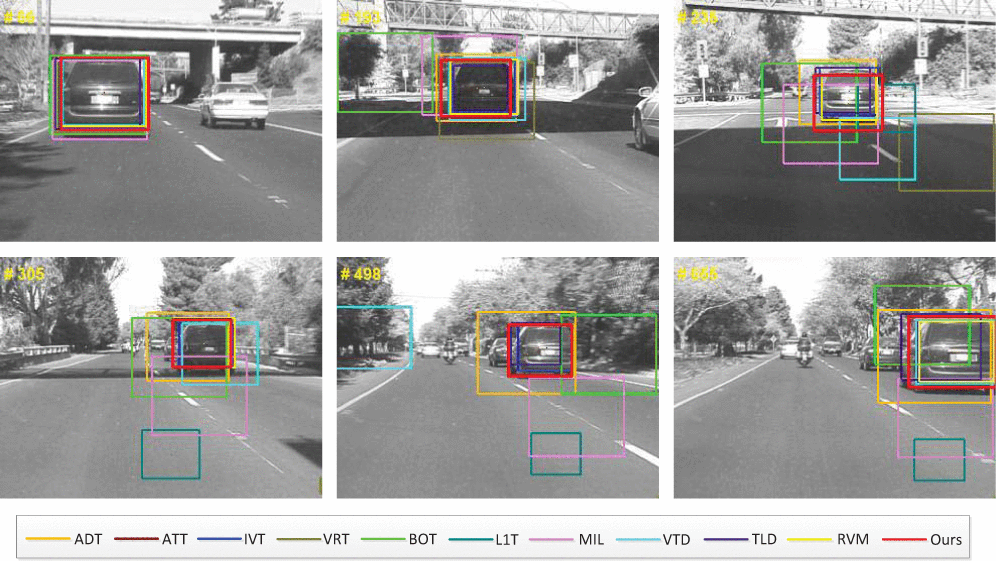
\includegraphics[width=1\textwidth]{tracking}
\caption{Frames from a tracking sequence featuring the bounding boxes indicating results
         of several tracking algorithms. Some examples of drift from the target and
         complete tracking failure can also be observed from some of the boxes.
         Source: Wang et.~al.~fig.~6~\cite{OBJECT_PLS}}\label{fig:tracking}
\end{figure}

\subsection{Target representation}
Early influential works in the field have used target models including subspaces
~\cite{EIGENTRACK} and representing the target as a curve~\cite{CONDENSATION}. Modern
tracking methods can be roughly divided to generative and discriminative, but combinations
of them have also been proposed.~\cite{DLT}

Generative methods search the frame for the best matches to a template of an appearance
model of the subject. Template methods based on pixel intensity and color histograms
perform well with no drastic changes in object appearance and non-cluttered backgrounds.
Appearance models learned from training can be less affected by appearance variations
and adaptive schemes provide added flexibility, while sparse models handle occlusion
and image noise better.~\cite{OBJECT_PLS}

Discriminative methods consider tracking as a binary classification problem. They take
the background also into account to separate the target from it. Used approaches
include refining the initial guess with a support vector machine~\cite{SVT} or utilizing
a relevance vector machine~\cite{SPARSE_BAYESIAN}.

During tracking, the appearance of the target may change for example due to changes in
orientation. Some trackers adapt the tracking model online to be robust against such
changes, but care must be taken in designing the update algorithm as it could result
to drift. Models using online updates have implemented it for example with results of
previous successful tracking results~\cite{BLUR_TRACK}.

\subsection{Datasets}
Research on networks working with image data has been made easier by larger sets of both
hand-labeled data and ones obtained by simple keyword searches from online image services.
With the adoption of unsupervised training and architectures not working as classifiers
unlabeled data can also be used to increase the size of the available training set.
The labeled resources introduced here consist of sets labeled with object classes contained
in the image or frame and ones for tracking with the target marked in each frame.

VOC was a yearly competition for object recognition and VOC 2012~\cite{VOC12} is the last
challenge in the series. The datasets of the challenges are still used for pre-training
features for detection stages in tracking networks. There are four major subsets of
hand-labeled VOC data: classification, segmentation action classification, person layout.
Classification datasets consist of images annotated with the objects contained and bounding
boxes for the objects drawn in the image itself while image segmentation sets provide
additional mask images of the objects and classes in each shot. Action classification sets
contain descriptions and bounding boxes of actions the subjects are performing and person
layout sets contain bounding boxes for the subject's head, hands and feet.
\authorcomment{image examples of the datasets, descriptions to annotations}

The \ac{ilsvrc}~\cite{ILSVRC15} is another recognition challenge running since 2010. The
most recent dataset consists of subsets of object localization, object detection and
object detection from video. The last subset is especially beneficial object tracking
tasks as it provides data for training on actual tracking data. The other two sets are also
substantially larger than the respective VOC sets as their labeling has been crowd sourced.

There has also been an increase in resources solely devoted to tracking data with the
TB-100 -set~\cite{VTB} being a good example. It contains a hundred tracking sequences
with reference positions for the target on each frame. Because some of the targets are
similar or less challenging, a subset of 50 sequences considered challenging is also
provided as TB-50.~\cite{OT_BENCH}

The datasets used for the \ac{vot}~\cite{VOT} can also be used for training networks. The competition
is run yearly with updated evaluation sets which can be used for training as training
data for a network but the challenge itself prohibits training on tracking datasets for
participants.

There is also the yearly \ac{mot}~\cite{MOT16} for testing multiple object trackers but
its unique sequences can also be used to train single object trackers one object at a
time.

\subsection{Evaluation}
Evaluation of proposed trackers is a vital part of the research. It also limits the use
of annotated tracking sequences in training as training and evaluation should be done
on different data.

The Visual Tracker Benchmark~\cite{VTB} is a commonly used resource for comparing
performance to other trackers. It consists of the TB-datasets, a code library containing
implementations of 31 publicly available trackers and ready benchmark results for the
included trackers. The code library is implemented using MATLAB and all included trackers
have been modified to use unified input and output formats. A Python-based testing suite
is also in development. The original benchmark was compiled in 2015 so doesn't include
more recent trackers in the suite. The \ac{vot}~\cite{VOT} and \ac{mot}~\cite{MOT16}
challenges also publish both the yearly challenge suite and results that can used to
compare new networks against the participants.

Precision and success plots are common metrics for comparing trackers against others.
Precision plot is the average center location error over the tracking sequence. This
error is calculated as the distance between the centers of the tracking location and
the hand-labeled ground truth. Success plot represents the average amount of overlap
and the bounding box to the ground truth in relation to their sizes. The overlap score
for a single frame is defined as the union of the boxes divided by their intersection.~\cite{OT_BENCH}
The raw errors can also be used in calculating other indicators. Used examples of these
are precision as the percentage of frames with a center distance error below a set value
and success rate as the percentage of frames with an overlap score above some threshold~\cite{DEEPTRACK}.
